\documentclass[12pt,a4paper]{article}
\usepackage[utf8]{inputenc}
\usepackage[portuguese]{babel}
\usepackage{geometry}
\usepackage{titlesec}
\usepackage{enumitem}
\usepackage{graphicx}

\geometry{margin=2.5cm}
\titleformat{\section}{\Large\bfseries}{\thesection}{1em}{}
\titleformat{\subsection}{\large\bfseries}{\thesubsection}{1em}{}

\title{\textbf{Processo de Gerenciamento de Projeto}\\
\large Sistema de Gestão de Feiras - Método Kanban}
\author{Higor Roger de Freitas Santos - 221006440\\
Victor Eneias Oliveira - 221038364\\
\\
Engenharia de Software CIC0105 Turma 01 2025.1}
\date{\today}

\begin{document}

\maketitle

\section{Ferramenta Utilizada}

Para o gerenciamento do projeto foi utilizado o método Kanban através da ferramenta GitHub Projects, que oferece integração direta com o repositório de código e interface web para organização das tarefas.

\begin{figure}[h]
    \centering
    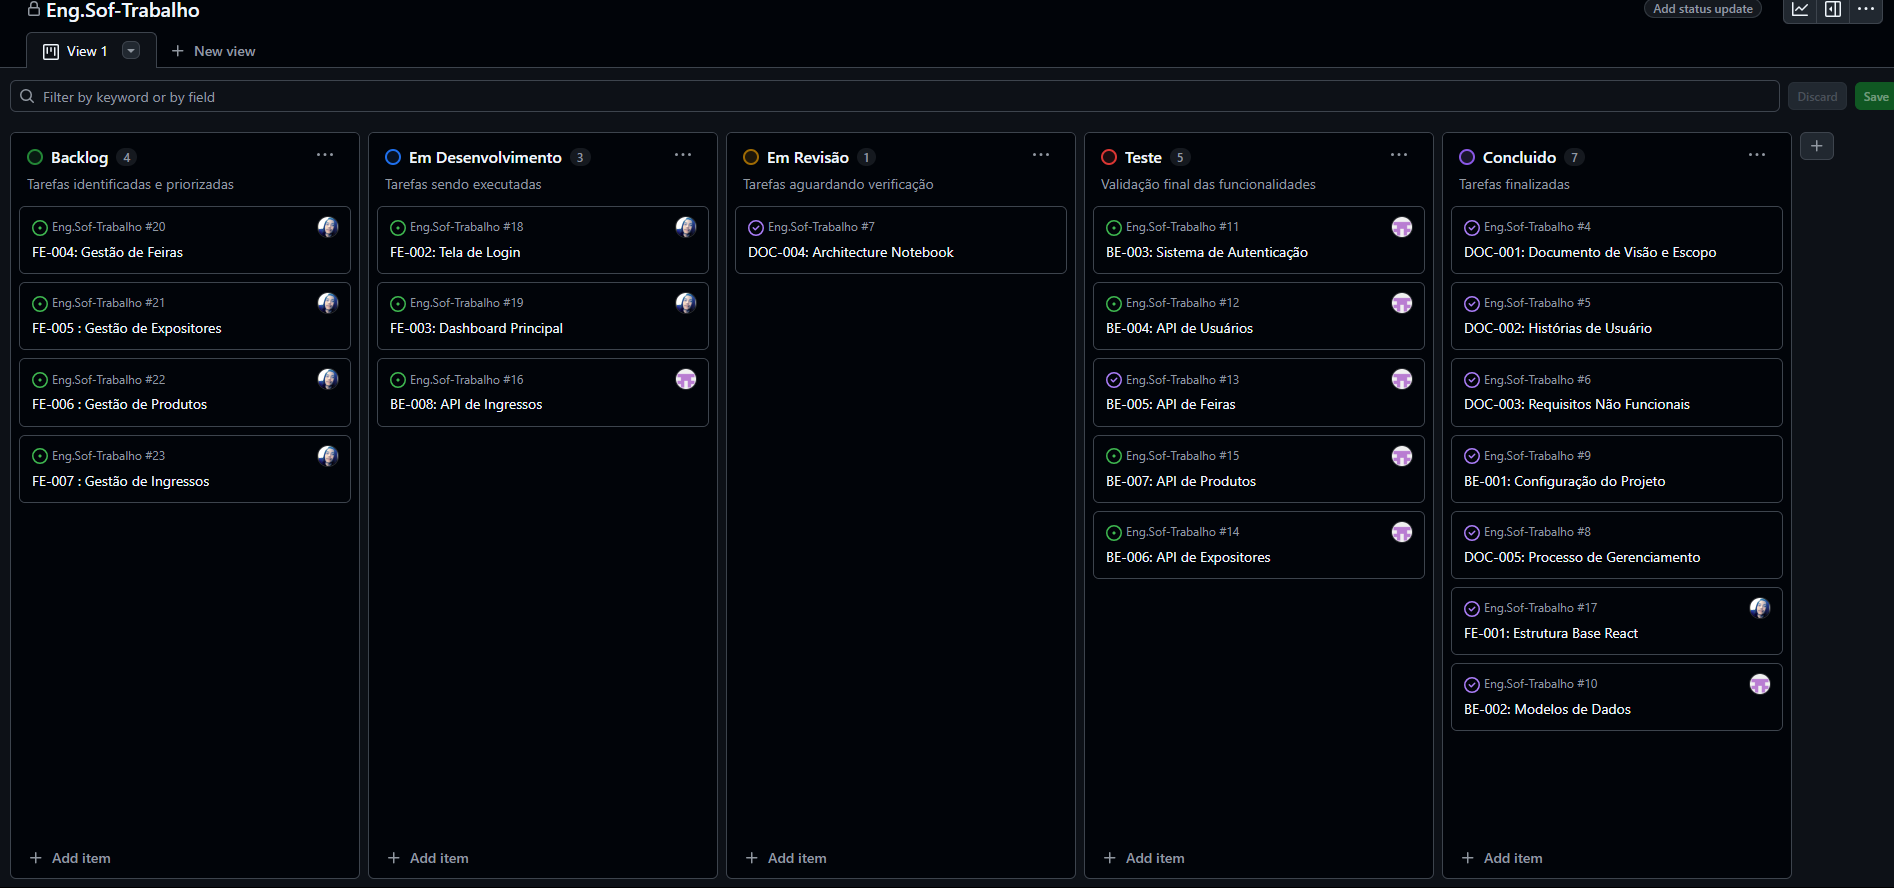
\includegraphics[width=0.9\textwidth]{processo/visao_geral_projeto.png}
    \caption{Visão geral do projeto no GitHub Projects}
    \label{fig:visao_geral}
\end{figure}

\section{Estrutura do Quadro Kanban}

O quadro foi organizado em 5 colunas para representar o fluxo de trabalho:

\begin{itemize}
    \item \textbf{Backlog}: Tarefas identificadas e priorizadas
    \item \textbf{Em Desenvolvimento}: Tarefas sendo executadas (máximo 3)
    \item \textbf{Em Revisão}: Tarefas aguardando verificação
    \item \textbf{Teste}: Validação final das funcionalidades
    \item \textbf{Concluído}: Tarefas finalizadas
\end{itemize}



\section{Cartões do Projeto}

Os cartões foram organizados por categorias usando labels para facilitar a identificação:

\begin{itemize}
    \item \textbf{documentation}: Documentação do projeto
    \item \textbf{backend}: Desenvolvimento do servidor
    \item \textbf{frontend}: Interface do usuário
    \item \textbf{database}: Banco de dados
    \item \textbf{testing}: Testes e validação
\end{itemize}

\begin{figure}[h]
    \centering
    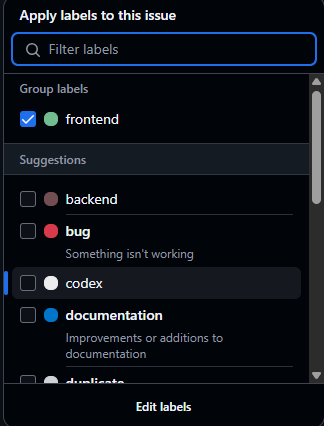
\includegraphics[width=0.3\textwidth]{processo/labels_github.png}
    \caption{Labels utilizadas para categorizar os cartões}
    \label{fig:labels}
\end{figure}

\subsection{Lista de Cartões Criados}

Foram criados 20 cartões organizados nas seguintes categorias:

\textbf{Documentação (5 cartões):}
\begin{itemize}
    \item DOC-001: Documento de Visão e Escopo
    \item DOC-002: Histórias de Usuário
    \item DOC-003: Requisitos Não Funcionais
    \item DOC-004: Architecture Notebook
    \item DOC-005: Processo de Gerenciamento
\end{itemize}



\textbf{Backend (8 cartões):}
\begin{itemize}
    \item BE-001: Configuração do Projeto
    \item BE-002: Modelos de Dados
    \item BE-003: Sistema de Autenticação
    \item BE-004: API de Usuários
    \item BE-005: API de Feiras
    \item BE-006: API de Expositores
    \item BE-007: API de Produtos
    \item BE-008: API de Ingressos
\end{itemize}



\textbf{Frontend (7 cartões):}
\begin{itemize}
    \item FE-001: Estrutura Base React
    \item FE-002: Tela de Login
    \item FE-003: Dashboard Principal
    \item FE-004: Gestão de Feiras
    \item FE-005: Gestão de Expositores
    \item FE-006: Gestão de Produtos
    \item FE-007: Gestão de Ingressos
\end{itemize}



\end{document}

    \textbf{BE-001: Configuração do Projeto}
    \begin{itemize}
        \item \textbf{Descrição}: Setup inicial do FastAPI, SQLAlchemy e estrutura de pastas
        \item \textbf{Critérios}: Projeto inicializa sem erros
        \item \textbf{Prioridade}: Alta
        \item \textbf{Estimativa}: 2 horas
    \end{itemize}

    \textbf{BE-002: Modelos de Dados}
    \begin{itemize}
        \item \textbf{Descrição}: Criar modelos SQLAlchemy para usuários, feiras, expositores, produtos e ingressos
        \item \textbf{Critérios}: Todos os modelos com relacionamentos corretos
        \item \textbf{Prioridade}: Alta
        \item \textbf{Estimativa}: 3 horas
    \end{itemize}

    \textbf{BE-003: Sistema de Autenticação}
    \begin{itemize}
        \item \textbf{Descrição}: Implementar login/registro com JWT
        \item \textbf{Critérios}: Autenticação funcionando com tokens seguros
        \item \textbf{Prioridade}: Alta
        \item \textbf{Estimativa}: 4 horas
    \end{itemize}

    \textbf{BE-004: API de Usuários}
    \begin{itemize}
        \item \textbf{Descrição}: Endpoints para registro, login e gestão de usuários
        \item \textbf{Critérios}: CRUD completo de usuários
        \item \textbf{Prioridade}: Alta
        \item \textbf{Estimativa}: 3 horas
    \end{itemize}

    \textbf{BE-005: API de Feiras}
    \begin{itemize}
        \item \textbf{Descrição}: Endpoints para CRUD de feiras com autorização
        \item \textbf{Critérios}: Apenas criador pode modificar feira
        \item \textbf{Prioridade}: Alta
        \item \textbf{Estimativa}: 3 horas
    \end{itemize}

    \textbf{BE-006: API de Expositores}
    \begin{itemize}
        \item \textbf{Descrição}: Endpoints para gestão de expositores vinculados a feiras
        \item \textbf{Critérios}: CRUD com validação de relacionamentos
        \item \textbf{Prioridade}: Média
        \item \textbf{Estimativa}: 3 horas
    \end{itemize}

    \textbf{BE-007: API de Produtos}
    \begin{itemize}
        \item \textbf{Descrição}: Endpoints para catálogo de produtos por expositor
        \item \textbf{Critérios}: CRUD com preços e descrições
        \item \textbf{Prioridade}: Média
        \item \textbf{Estimativa}: 3 horas
    \end{itemize}

    \textbf{BE-008: API de Ingressos}
    \begin{itemize}
        \item \textbf{Descrição}: Sistema de emissão e gestão de ingressos
        \item \textbf{Critérios}: Ingressos únicos por feira e data
        \item \textbf{Prioridade}: Média
        \item \textbf{Estimativa}: 2 horas
    \end{itemize}

    \subsubsection{Desenvolvimento Frontend}

    \textbf{FE-001: Estrutura Base React}
    \begin{itemize}
        \item \textbf{Descrição}: Setup do React.js com componentes principais
        \item \textbf{Critérios}: Interface básica funcionando
        \item \textbf{Prioridade}: Alta
        \item \textbf{Estimativa}: 2 horas
    \end{itemize}

    \textbf{FE-002: Tela de Login}
    \begin{itemize}
        \item \textbf{Descrição}: Interface para login e registro de usuários
        \item \textbf{Critérios}: Formulários funcionais com validação
        \item \textbf{Prioridade}: Alta
        \item \textbf{Estimativa}: 3 horas
    \end{itemize}

    \textbf{FE-003: Dashboard Principal}
    \begin{itemize}
        \item \textbf{Descrição}: Tela principal com navegação entre módulos
        \item \textbf{Critérios}: Menu funcional e responsivo
        \item \textbf{Prioridade}: Alta
        \item \textbf{Estimativa}: 2 horas
    \end{itemize}

    \textbf{FE-004: Gestão de Feiras}
    \begin{itemize}
        \item \textbf{Descrição}: Interface para CRUD de feiras
        \item \textbf{Critérios}: Listagem, criação, edição e exclusão
        \item \textbf{Prioridade}: Alta
        \item \textbf{Estimativa}: 4 horas
    \end{itemize}

    \textbf{FE-005: Gestão de Expositores}
    \begin{itemize}
        \item \textbf{Descrição}: Interface para gestão de expositores
        \item \textbf{Critérios}: CRUD vinculado a feiras
        \item \textbf{Prioridade}: Média
        \item \textbf{Estimativa}: 3 horas
    \end{itemize}

    \textbf{FE-006: Gestão de Produtos}
    \begin{itemize}
        \item \textbf{Descrição}: Interface para catálogo de produtos
        \item \textbf{Critérios}: CRUD com preços e imagens
        \item \textbf{Prioridade}: Média
        \item \textbf{Estimativa}: 3 horas
    \end{itemize}

    \textbf{FE-007: Gestão de Ingressos}
    \begin{itemize}
        \item \textbf{Descrição}: Interface para emissão de ingressos
        \item \textbf{Critérios}: Geração e listagem de ingressos
        \item \textbf{Prioridade}: Média
        \item \textbf{Estimativa}: 2 horas
    \end{itemize}

    \subsubsection{Testes e Qualidade}

    \textbf{TEST-001: Testes de API}
    \begin{itemize}
        \item \textbf{Descrição}: Criar testes automatizados para endpoints
        \item \textbf{Critérios}: Cobertura de cenários principais
        \item \textbf{Prioridade}: Média
        \item \textbf{Estimativa}: 4 horas
    \end{itemize}

    \textbf{TEST-002: Testes de Interface}
    \begin{itemize}
        \item \textbf{Descrição}: Validar funcionamento da interface
        \item \textbf{Critérios}: Fluxos principais testados
        \item \textbf{Prioridade}: Média
        \item \textbf{Estimativa}: 3 horas
    \end{itemize}

    \textbf{TEST-003: Vídeo de Demonstração}
    \begin{itemize}
        \item \textbf{Descrição}: Gravar demonstração completa do sistema
        \item \textbf{Critérios}: Todos os cenários de sucesso mostrados
        \item \textbf{Prioridade}: Baixa
        \item \textbf{Estimativa}: 2 horas
    \end{itemize}

    \section{Fluxo de Trabalho}

    \subsection{Processo Padrão}

    \begin{enumerate}
        \item \textbf{Planejamento}: Cartões criados no Backlog
        \item \textbf{Desenvolvimento}: Movidos para "Em Desenvolvimento"
        \item \textbf{Revisão}: Código/documento revisado
        \item \textbf{Teste}: Validação funcional
        \item \textbf{Conclusão}: Tarefa finalizada
    \end{enumerate}

    \subsection{Regras do Quadro}

    \begin{itemize}
        \item Máximo 3 cartões em "Em Desenvolvimento"
        \item Todo cartão deve ter critérios de aceitação
        \item Revisão obrigatória antes dos testes
        \item Documentação atualizada a cada entrega
    \end{itemize}

    \section{Métricas e Acompanhamento}

    \subsection{Métricas Coletadas}

    \textbf{Lead Time}: Tempo desde criação até conclusão do cartão
    \textbf{Cycle Time}: Tempo desde início do desenvolvimento até conclusão
    \textbf{Throughput}: Número de cartões concluídos por semana
    \textbf{WIP}: Quantidade de trabalho em progresso

    \subsection{Relatórios}

    O GitHub Projects gera automaticamente:
    \begin{itemize}
        \item Burndown chart do projeto
        \item Velocity da equipe
        \item Distribuição de trabalho por categoria
        \item Tempo médio por tipo de tarefa
    \end{itemize}

    \section{Benefícios Obtidos}

    \subsection{Visibilidade}
    \begin{itemize}
        \item Status claro de cada tarefa
        \item Progresso visual do projeto
        \item Identificação de gargalos
    \end{itemize}

    \subsection{Flexibilidade}
    \begin{itemize}
        \item Priorização dinâmica
        \item Adaptação a mudanças
        \item Fluxo contínuo de entrega
    \end{itemize}

    \subsection{Qualidade}
    \begin{itemize}
        \item Revisão obrigatória
        \item Testes sistemáticos
        \item Critérios claros de conclusão
    \end{itemize}

    \section{Conclusão}

    O método Kanban implementado através do GitHub Projects mostrou-se adequado para o gerenciamento do projeto acadêmico, proporcionando organização, visibilidade e controle sobre o desenvolvimento. A integração com o repositório Git facilitou a rastreabilidade entre tarefas e código, contribuindo para a qualidade final do sistema.

    A estrutura de 5 colunas e 22 cartões permitiu um fluxo organizado de trabalho, desde a concepção até a entrega, garantindo que todos os artefatos solicitados fossem desenvolvidos de forma sistemática e controlada.

    \end{document} 